% \part{Projeto}

\chapter[Projeto]{Projeto}

\section{Requisitos}

Para o desenvolvimento do projeto de uma arquitetura de Data Fabric para salvar imagens de câncer de pele, foram definidos os seguintes requisitos:

\subsection{Requisitos Funcionais}
\begin{table}[H]
    \centering
    \begin{tabular}{|c|p{12cm}|}
    \hline
    \textbf{ID} & \textbf{Requisito} \\ \hline
    RFSO01 & O sistema deve ser capaz de armazenar grandes volumes de imagens de câncer de pele. \\ \hline
    RFSO02 & O sistema deve permitir o processamento eficiente das imagens armazenadas. \\ \hline
    RFSO03 & O sistema deve garantir a segurança e a privacidade dos dados dos pacientes. \\ \hline
    RFSO04 & Os dados devem estar disponíveis para acesso por pesquisadores e profissionais de saúde de forma segura. \\ \hline
    RFSO05 & O sistema deve ser escalável para acomodar o aumento no volume de dados ao longo do tempo. \\ \hline
    RFSO06 & O sistema deve permitir o compartilhamento seguro de dados utilizando Delta Sharing. \\ \hline
    RFSO07 & O sistema deve permitir a integração de dados de diferentes fontes de forma unificada. \\ \hline
    RFSO08 & O sistema deve oferecer uma camada de virtualização para consulta de dados distribuídos. \\ \hline
    RFSO09 & O sistema deve permitir a governança centralizada dos dados, com controle de acesso baseado em papéis. \\ \hline
    RFSO10 & O sistema deve suportar análises em tempo real para dados armazenados e em trânsito. \\ \hline
    RFSO11 & O sistema deve possuir uma camada de metadados para catalogação de imagens e dados relacionados. \\ \hline
    RFSO12 & O sistema deve fornecer APIs para facilitar a integração com ferramentas de visualização de dados. \\ \hline
    \end{tabular}
    \caption{Tabela de Requisitos Funcionais}
    \label{tab:requisitos_funcionais}
\end{table}

\subsection{Requisitos Não Funcionais}
\begin{table}[H]
    \centering
    \begin{tabular}{|c|p{12cm}|}
    \hline
    \textbf{ID} & \textbf{Requisito} \\ \hline
    RNFSO01 & O sistema deve ser capaz de processar e recuperar dados rapidamente. \\ \hline
    RNFSO02 & O sistema deve garantir a integridade e a consistência dos dados armazenados. \\ \hline
    RNFSO03 & A interface do sistema deve ser intuitiva e fácil de usar para os profissionais de saúde. \\ \hline
    RNFSO04 & O sistema deve ser de fácil manutenção e atualização. \\ \hline
    RNFSO05 & A arquitetura deve ser modular para facilitar a expansão e substituição de componentes. \\ \hline
    RNFSO06 & O sistema deve oferecer suporte a padrões de interoperabilidade, como FHIR. \\ \hline
    RNFSO07 & O sistema deve garantir compatibilidade com regulamentações de proteção de dados, como LGPD. \\ \hline
    \end{tabular}
    \caption{Tabela de Requisitos Não Funcionais}
    \label{tab:requisitos_nao_funcionais}
\end{table}

\subsection{Histórias de Usuário}
\begin{table}[H]
    \centering
    \begin{tabular}{|c|p{8cm}|c|c|}
    \hline
    \textbf{Requisitos} & \textbf{Descrição} & \textbf{MoSCoW} & \textbf{Pontuação} \\ \hline
    RFSO01 & Como pesquisador, quero armazenar grandes volumes de imagens de câncer de pele para análise. & Must Have & 8 \\ \hline
    RFSO03 & Como administrador, quero garantir a privacidade dos dados dos pacientes armazenados. & Must Have & 9 \\ \hline
    RFSO04 & Como médico, quero acessar dados de forma segura para apoiar o diagnóstico. & Must Have & 8 \\ \hline
    RFSO06 & Como pesquisador, quero compartilhar dados de forma segura com outras organizações ou contribuidores. & Should Have & 7 \\ \hline
    RFSO07 & Como administrador, quero integrar dados de diferentes bases de dados para análise centralizada. & Must Have & 9 \\ \hline
    RFSO08 & Como pesquisador, quero consultar dados distribuídos sem me preocupar com a origem física dos dados. & Should Have & 7 \\ \hline
    RFSO09 & Como administrador, quero controlar acessos de forma centralizada para garantir segurança. & Must Have & 8 \\ \hline
    RFSO10 & Como pesquisador, quero realizar análises em tempo real para melhorar a precisão dos resultados. & Could Have & 6 \\ \hline
    RFSO11 & Como desenvolvedor, quero acessar um catálogo centralizado de metadados para identificar rapidamente os dados necessários. & Should Have & 7 \\ \hline
    RNFSO07 & Como administrador, quero garantir que os dados do sistema estejam em conformidade com LGPD. & Must Have & 10 \\ \hline
    \end{tabular}
    \caption{Tabela de Histórias de Usuário}
    \label{tab:historias_usuario}
\end{table}

\section{Arquitetura}

A arquitetura do projeto será baseada na abordagem de Data Fabric, que permite a integração e gestão de dados de forma unificada e eficiente. A seguir, a descrição dos principais componentes da arquitetura:

\subsection{Diagrama de Arquitetura}
A figura \ref{fig:arquitetura_projeto} ilustra a arquitetura proposta, cujo núcleo é o Data Fabric, responsável por integrar fontes de dados internas e externas, incluindo Google Cloud Storage, MongoDB e bancos de dados relacionais. O MinIO funciona como a fonte interna de armazenamento, dividida nas camadas Bronze, Silver e Gold, que suportam, respectivamente, a inserção inicial, o pré-processamento e o enriquecimento dos dados. A ingestão se inicia por meio de uma DAG de inserção gerenciada pelo Apache Airflow, que realiza coleta (scraping) de imagens de câncer de pele em diferentes repositórios, armazenando-as na camada Bronze do Data Lake (MinIO) junto a seus metadados, os quais são registrados no Delta Lake. Em seguida, ocorre uma nova etapa coordenada por outra DAG do Apache Airflow, na qual o pré-processamento e a análise das imagens são executados, resultando em dados enriquecidos que passam a compor as camadas Silver ou Gold no MinIO, ao mesmo tempo em que o Delta Lake mantém a organização e o controle de versões dos metadados. O Spark atua como motor de processamento que aproveita a camada transacional do Delta Lake para garantir integridade (ACID) e versionamento, além de oferecer as ferramentas necessárias para manipular ou analisar grandes volumes de informações. Por fim, o Delta Sharing possibilita a disponibilização desses dados de maneira segura a pesquisadores e organizações, preservando a governança e a privacidade das informações.

\begin{figure}[h]
    \centering
    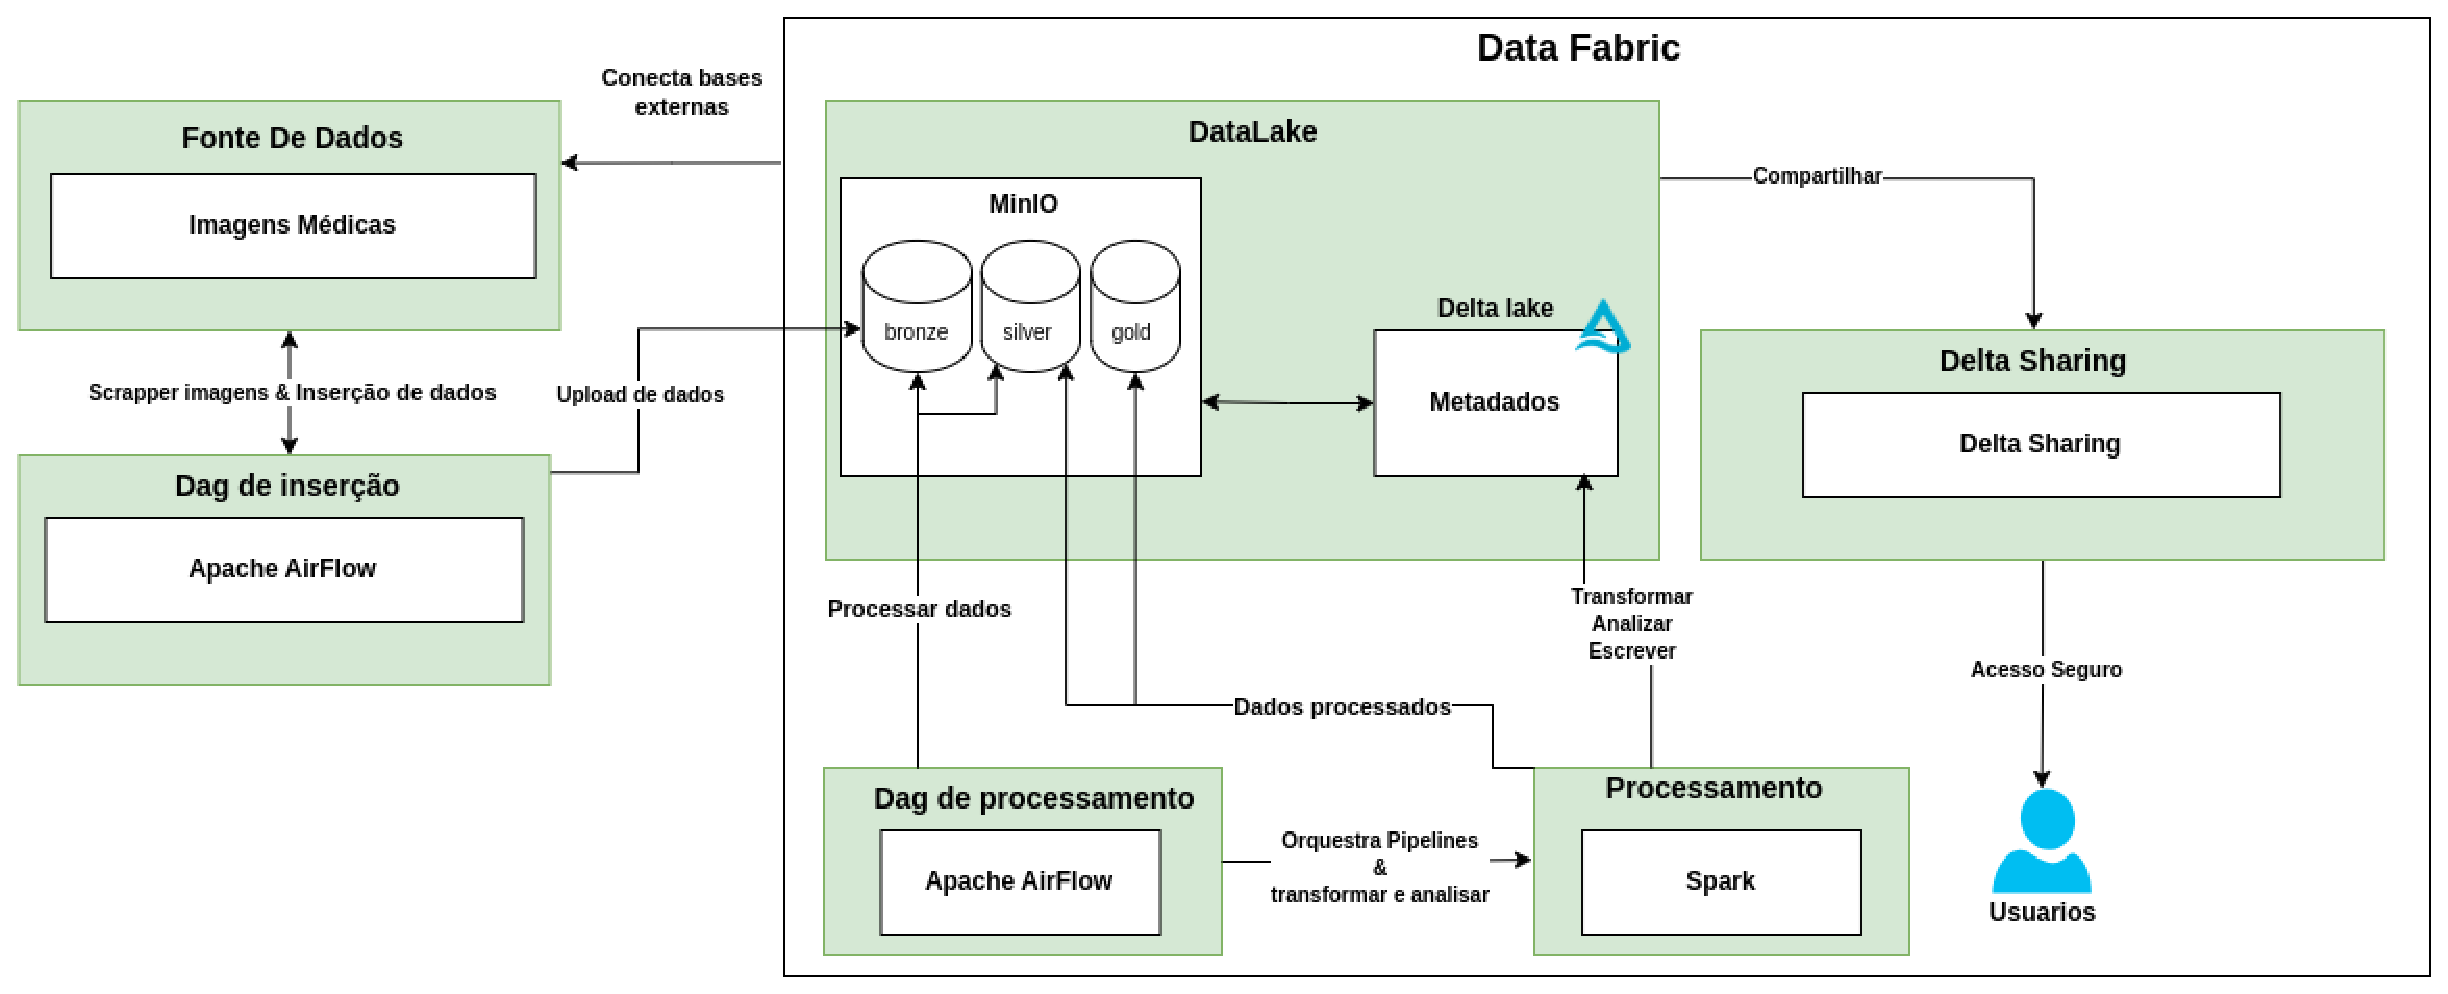
\includegraphics[width=0.8\textwidth]{figuras/arquitetura.eps}
    \caption{Diagrama da Arquitetura do Projeto }
    \label{fig:arquitetura_projeto}
\end{figure} 


\subsection{Diagrama de Fluxo de Dados}
A figura \ref{fig:fluxo_dados_projeto} ilustra um fluxo de dados em que múltiplas fontes (como hospitais, pesquisas colaborativas e repositórios de imagens médicas) alimentam o sistema por meio de uma DAG de inserção, orquestrada pelo Apache Airflow. Essa etapa controla a ingestão de arquivos e seus metadados, direcionando-os ao DataLake, no qual o MinIO provê armazenamento distribuído. Paralelamente, o Delta Lake é responsável por gerenciar as informações de metadados e garantir versionamento e rastreabilidade das atualizações. Na sequência, uma segunda fase de orquestração ocorre na etapa de Processamento de Dados, na qual o próprio Apache Airflow ativa as rotinas de pré-processamento e de análise, empregando o Spark especificamente para transformações nos metadados e extração de insights. Com os dados processados, o sistema conta com um módulo de Governança e Segurança que adota políticas de controle de acesso (RBAC) e está em conformidade com a LGPD, assegurando integridade e privacidade das informações médicas. Por fim, o módulo de Compartilhamento de Dados, apoiado no Delta Sharing, facilita o acesso seguro a pesquisadores e outras organizações, permitindo consultas autorizadas e promovendo a colaboração em larga escala.

\begin{figure}[h]
    \centering
    \includegraphics[width=0.8\textwidth]{figuras/diagrama_fluxo_dados.eps}
    \caption{Diagrama da Fluxo de Dados }
    \label{fig:fluxo_dados_projeto}
\end{figure} 



\subsection{Componentes da Arquitetura}
\begin{itemize}
    \item \textbf{Ingestão de Dados}: Utilização de pipelines de ingestão para coletar e armazenar imagens de câncer de pele de diversas fontes (hospitais, clínicas, pesquisas).
    \item \textbf{Armazenamento de Dados}: Implementação de um sistema de armazenamento distribuído, como MinIO, para garantir a escalabilidade e a disponibilidade das imagens.
    \item \textbf{Processamento de Dados}: Utilização de ferramentas como Apache Airflow para a orquestração de pipelines de processamento das imagens.
    \item \textbf{Gestão de Dados}: Aplicação de Data Fabric para fornecer uma camada de abstração que facilita a integração e gestão dos dados distribuídos.
    \item \textbf{Compartilhamento de Dados}: Utilização de Delta Sharing para permitir o compartilhamento seguro de dados entre diferentes organizações.
    \item \textbf{Interface de Usuário}: Desenvolvimento de uma interface web utilizando FastAPI para permitir o acesso e a manipulação dos dados por pesquisadores e profissionais de saúde.
\end{itemize}

\subsection{Fluxo de Dados}
\begin{itemize}
    \item \textbf{Coleta e Ingestão}: As imagens são coletadas de diversas fontes e armazenadas no sistema de armazenamento distribuído.
    \item \textbf{Processamento}: As imagens armazenadas são processadas através de pipelines orquestrados pelo Apache Airflow, que podem incluir etapas de pré-processamento, análise e extração de características.
    \item \textbf{Armazenamento e Gestão}: Os dados processados são armazenados e geridos pela arquitetura de Data Fabric, que garante a integração e a consistência dos dados.
    \item \textbf{Compartilhamento de Dados}: Utilizando Delta Sharing, os dados podem ser compartilhados de forma segura com outras organizações e pesquisadores.
    \item \textbf{Acesso aos Dados}: A interface web desenvolvida com FastAPI permite que os usuários acessem e manipulem os dados de forma segura e eficiente.
\end{itemize}

\section{Tecnologias Utilizadas}

Com base no referencial teórico, as seguintes tecnologias serão utilizadas no projeto:
\begin{itemize}
    \item \textbf{MinIO}: Para o armazenamento distribuído das imagens, garantindo escalabilidade e disponibilidade.
    \item \textbf{Apache Airflow}: Para a orquestração de pipelines de processamento de dados.
    \item \textbf{Data Fabric}: Para a integração e gestão de dados de forma unificada.
    \item \textbf{Delta Sharing}: Para o compartilhamento seguro de dados entre diferentes organizações.
    \item \textbf{FastAPI}: Para o desenvolvimento da interface web, permitindo o acesso e a manipulação dos dados.
    \item \textbf{Kubernetes}: Para a orquestração de containers, garantindo a escalabilidade e a alta disponibilidade do sistema.
    \item \textbf{Spark}: Fornece um alto nível de paralelismo, processando grandes quantidades de dados eficientimente em vários nós em um cluster.
\end{itemize}

\section{Roadmap de Implementação}

A implementação dessa arquitetura será conduzida em etapas sequenciais, cada qual associada a um intervalo de tempo estimado, de modo a garantir uma implantação organizada e confiável. Inicialmente, dedica-se um período de aproximadamente duas semanas à configuração do ambiente de desenvolvimento e à implantação do cluster Kubernetes, estabelecendo a infraestrutura necessária para a orquestração e o provisionamento de contêineres. Na sequência, com o Kubernetes já operacional, realiza-se a configuração do MinIO para armazenamento distribuído de dados brutos.; essas tarefas, que incluem testes iniciais de integração, tendem a demandar mais uma ou duas semanas.

Em seguida, procede-se à instalação e integração do Delta Lake com MiniO, fundamental para o versionamento e a gestão transacional dos dados, o que costuma levar cerca de uma semana, considerando a adequação às políticas de governança que regem os metadados. Logo após, configura-se o Apache Airflow, que assume o papel de orquestração das DAGs de inserção e de processamento. A etapa de implantação e ajuste das pipelines, contemplando definição de dependências, verificação de logs e testes de escalabilidade, durando de duas a três semanas.

Por fim, entra-se na fase de implementação do Delta Sharing, que inclui ajustes de segurança (por exemplo, RBAC para controle de acesso e conformidade com a LGPD) e finaliza o ciclo de entrega, em mais duas semanas. Nessa etapa, os recursos de compartilhamento seguro de dados são configurados e submetidos a validações de desempenho e de governança, assegurando que apenas usuários e organizações devidamente autorizados tenham acesso à informação. Após esse período, será realizadas verificações integradas em todo o ecossistema, incluindo testes de carga e monitoramento contínuo, assegurando uma solução robusta, escalável e pronta para suportar o processamento e a análise de grandes volumes de dados de maneira confiável.